\documentclass[11pt,a4paper]{article}

\usepackage[margin=2.15cm]{geometry}
\usepackage{booktabs}
\usepackage{amsmath}
\usepackage{amssymb}
\usepackage{microtype}
\usepackage[hidelinks]{hyperref}
\usepackage{enumitem}
\usepackage{listings}
\usepackage{tikz}
\lstset{
  basicstyle=\ttfamily\scriptsize,
  breaklines=true,
  columns=fullflexible,
  frame=single,
  aboveskip=0.5em,
  belowskip=0.5em,
  xleftmargin=0.4em,
  xrightmargin=0.4em
}
\usetikzlibrary{arrows.meta,positioning,fit,backgrounds}
\setlist{nosep,leftmargin=1.35em}
\setlength{\parskip}{0.35em}
\setlength{\parindent}{0pt}

\title{RiskSphere\\[0.25em]
\large A multi-agent desk for counterparty risk, collateral, and clause retrieval}
\author{RiskSphere}
\date{22 November 2026}

\begin{document}
\maketitle
\vspace{-1.6em}
\begin{abstract}
\noindent
RiskSphere answers questions about a synthetic six-name book. Each credit limit is that name's simulated collateralised peak, times a factor, rounded. Two agents call Qwen/Qwen3-8B. The orchestrator plans the question and writes the sentences. Documents reads one retrieved clause when the question asks for an agreement number. Python computes exposure, margin, the simulation, scenarios, coverage, expected loss, and the desk files, and it checks every quote. The filing folders hold 522 credit-support texts, 278 contracts, 150 disclosure excerpts, and the BCBS margin text. A term extracted from an agreement is verified only when the quote is in the file. A critic written in Python drops any sentence whose number, status, or citation is not in the tool result. The frozen question set is 27 rows, with duplicate questions removed. On the live run of 22 November 2026, 14:42 IST, the plan was right on 25 of 27, every refusal was correct, and the critic rejected 8 of 21 wordings.
\end{abstract}

\section{Problem and boundary}

A collateral desk asks a small set of questions. What is the exposure today? Is the name through its limit? What margin is due? What does the agreement say the threshold is? What happens if equities fall? A wrong number is worse than no answer. An 8B chat model is a poor calculator: it rounds, it mixes today's exposure with a simulated future exposure, and it quotes an agreement sentence it was never shown. It is useful at one job, which is choosing the calculation and then writing a short note once the numbers exist.

The book is illustrative and has six names. Trades and agreement terms were written for the project. Each credit limit is the simulated collateralised peak times a factor, rounded. Prices are live Yahoo daily closes. If Yahoo does not answer, the question stops. An older saved close is not substituted. The labelled retrieval set is sample text in two piles. The term sheet is extracted from downloaded EDGAR agreements, and a field is verified only when the quote is in the file.

Three labels are fixed and are checked in the wording. The future-exposure number is a prototype simulation, not Basel SA-CCR. The initial-margin number is a normal-loss proxy, not ISDA SIMM. Expected loss uses a synthetic probability of default and loss given default. It is not regulatory exposure at default, and those rates are not inferred from a company name.

The action boundary is equally fixed. The system calculates a delivery or a return and can write a draft notice, a draft report, a draft stress book, a draft dispute row, or a draft term. It does not send, approve, release, book, pay, or change a stored limit. A person signs off somewhere else. Every draft file is marked \texttt{DRAFT\_PENDING\_APPROVAL}, and \texttt{applied} stays false.

\section{Architecture}

Two agents, and both call Qwen. The orchestrator owns no formula. It runs the guardrails, asks Qwen for one JSON plan of at most four steps, dispatches each step, asks Qwen for sentences, and runs the critic. Documents is the second agent. It retrieves clauses. When the question asks for a threshold, a minimum transfer amount, a rounding amount, or an independent amount, Documents asks Qwen to copy one quote and name one amount. Python then runs the quote gate, and a draft is written only when that gate returns verified. Each remaining tool belongs to exactly one Python service, and that service does not call the model. The map from tool name to owner is the single list, so the log line, the dispatcher, and this report cannot drift apart. A formula, a workbook, or a notice stays in Python.

\begin{figure}[ht]
\centering
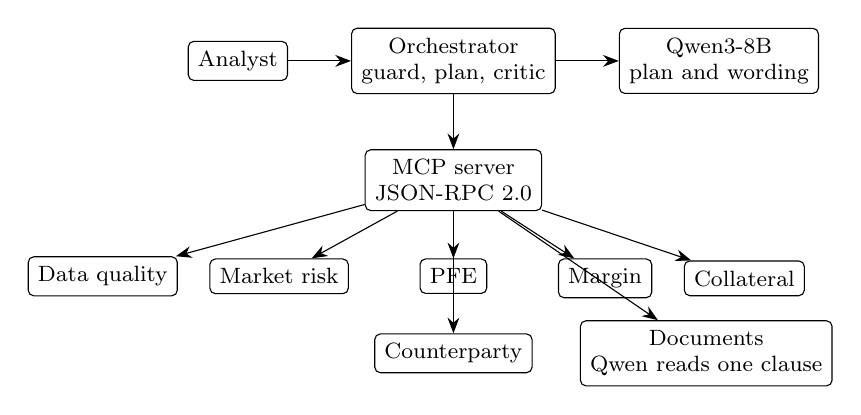
\begin{tikzpicture}[
  font=\footnotesize,
  box/.style={draw, rounded corners=2pt, align=center, inner sep=3.5pt, fill=white},
  >={Stealth[length=2mm]}
]
  \node[box] (user) {Analyst};
  \node[box, right=8mm of user] (orch) {Orchestrator\\guard, plan, critic};
  \node[box, right=8mm of orch] (qwen) {Qwen3-8B\\plan and wording};
  \node[box, below=7mm of orch] (mcp) {MCP server\\JSON-RPC 2.0};
  \node[box, below left=6mm and 2mm of mcp] (mkt) {Market risk};
  \node[box, below=6mm of mcp] (pfe) {PFE};
  \node[box, below right=6mm and 2mm of mcp] (mar) {Margin};
  \node[box, left=4mm of mkt] (dq) {Data quality};
  \node[box, right=4mm of mar] (col) {Collateral};
  \node[box, below=5mm of pfe] (cp) {Counterparty};
  \node[box, right=6mm of cp] (doc) {Documents\\Qwen reads one clause};
  \draw[->] (user) -- (orch);
  \draw[->] (orch) -- (qwen);
  \draw[->] (orch) -- (mcp);
  \draw[->] (mcp) -- (dq);
  \draw[->] (mcp) -- (mkt);
  \draw[->] (mcp) -- (pfe);
  \draw[->] (mcp) -- (mar);
  \draw[->] (mcp) -- (col);
  \draw[->] (mcp) -- (cp);
  \draw[->] (mcp) -- (doc);
\end{tikzpicture}
\caption{Two agents call Qwen. The orchestrator plans and phrases. Documents reads one retrieved clause and proposes a term. Python checks the quote. The other boxes are Python, reached by an MCP \texttt{tools/call} after a plan exists. They do not call the model and they do not call each other.}
\end{figure}

The console does not evaluate the formulas. After validation, each step is a \texttt{tools/call} on a child process. The transport is JSON-RPC 2.0, protocol version \texttt{2024-11-05}, one JSON object per line on standard input and output. Server logs go to standard error so a log line cannot be parsed as a protocol message. The methods used are \texttt{initialize}, \texttt{notifications/initialized}, \texttt{tools/list}, \texttt{tools/call}, and \texttt{ping}. Qwen never speaks MCP. The orchestrator does, and only after it already has a plan.

The chat gateway allows one active request. The plan, a Documents reading, and the wording share a lock. A 429 or a 503 waits 2\,s, then 4\,s, then 8\,s. TLS verification stays on. The key is read from a local file that is not committed, and it is never written to the trace.

\section{Sequence of one question}

Nothing is calculated until a question is typed. The same process remembers the last counterparty, so a later question can say ``its'' and still mean that name. A question over 1{,}000 characters is rejected before the guardrails. A later step does not start if an earlier step already stopped the question.

\begin{figure}[ht]
\centering
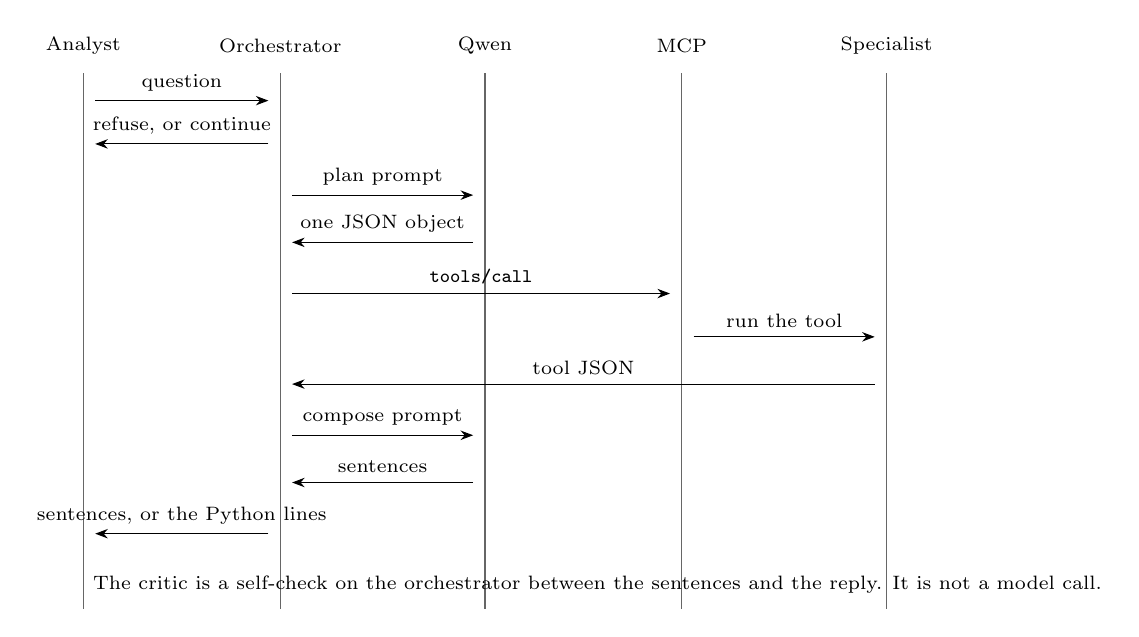
\begin{tikzpicture}[
  font=\scriptsize,
  every node/.style={align=center},
  lifeline/.style={draw=black!60},
  >={Stealth[length=1.6mm]}
]
  \foreach \n/\x in {Analyst/0, Orchestrator/2.5, Qwen/5.1, MCP/7.6, Specialist/10.2} {
    \node (\n) at (\x,0) {\n};
    \draw[lifeline] (\x,-0.35) -- (\x,-7.15);
  }
  \draw[->] (0.15,-0.7) -- (2.35,-0.7) node[midway, above] {question};
  \draw[->] (2.35,-1.25) -- (0.15,-1.25) node[midway, above] {refuse, or continue};
  \draw[->] (2.65,-1.9) -- (4.95,-1.9) node[midway, above] {plan prompt};
  \draw[->] (4.95,-2.5) -- (2.65,-2.5) node[midway, above] {one JSON object};
  \draw[->] (2.65,-3.15) -- (7.45,-3.15) node[midway, above] {\texttt{tools/call}};
  \draw[->] (7.75,-3.7) -- (10.05,-3.7) node[midway, above] {run the tool};
  \draw[->] (10.05,-4.3) -- (2.65,-4.3) node[midway, above] {tool JSON};
  \draw[->] (2.65,-4.95) -- (4.95,-4.95) node[midway, above] {compose prompt};
  \draw[->] (4.95,-5.55) -- (2.65,-5.55) node[midway, above] {sentences};
  \draw[->] (2.35,-6.2) -- (0.15,-6.2) node[midway, above] {sentences, or the Python lines};
  \node[anchor=west] at (0,-6.85) {The critic is a self-check on the orchestrator between the sentences and the reply. It is not a model call.};
\end{tikzpicture}
\caption{Sequence for a question that passes the guardrails. A refusal returns on the second arrow and never reaches Qwen or MCP.}
\end{figure}

If the plan came from a failed JSON parse, or the model was not called, there is no wording call. The Python lines are the answer. If the plan came from Qwen and at least one tool succeeded, the compose call runs. The critic may send the same prompt back once, with the failure names appended. A second failure discards the sentences.

\section{How the agents are used}

The orchestrator does not pick an owner by name. It picks a tool. The map then names Documents or a Python service, and the console log prints that name while the tool runs. Documents and the services do not talk to each other. A Python service does not call the model. Documents calls Qwen only after retrieval, and only to propose one term. A question may plan up to four tools, for example a data-quality check and then today's exposure, or a clause search. They read the book, Yahoo, or the clause corpus, and they return JSON.

\begin{center}
\begin{tabular}{@{}lp{9.6cm}@{}}
\toprule
Owner & Tools \\
\midrule
Orchestrator (agent) & none; guardrails, plan, wording, critic \\
Documents (agent) & \texttt{search\_clauses}, \texttt{propose\_term} \\
Data quality (Python) & \texttt{check\_data\_quality} \\
Market (Python) & \texttt{get\_market\_data}, \texttt{scenario\_pnl}, \texttt{draft\_stress\_book} \\
Simulation (Python) & \texttt{check\_pfe\_limit} \\
Margin (Python) & \texttt{calculate\_margin\_call}, \texttt{initial\_margin\_proxy}, \texttt{draft\_margin\_notice} \\
Collateral (Python) & \texttt{regulatory\_haircut}, \texttt{collateral\_coverage} \\
Exposure (Python) & \texttt{current\_exposure}, \texttt{expected\_loss}, \texttt{list\_alerts}, \texttt{draft\_dispute}, \texttt{draft\_report} \\
\bottomrule
\end{tabular}
\end{center}

What each calculation is, at the level the critic later checks:

\begin{itemize}
  \item Today's exposure. For trade $i$, mark $q_i(S_i-K_i)$ from the last close $S_i$ and the stored entry $K_i$. Eligible collateral is face times $(1-h)$, with $h$ the schedule haircut. Exposure is $\max(\sum \mathrm{mark} - C,\, 0)$. Utilization is that exposure over the stored limit. Above 100\% the status is \texttt{BREACH}. From 85\% inclusive it is \texttt{WARNING}. Otherwise \texttt{OK}. The status uses the unrounded ratio. The shown percent is one decimal.
  \item Variation margin. Credit support is $\max(0,\, \mathrm{MTM}+\mathrm{IA}-\mathrm{threshold})$. The raw delivery is credit support minus eligible collateral. At or above the minimum transfer amount, a delivery rounds up to the agreement step and a return rounds down. Below the minimum transfer, the action is no action. Any delivery or return is flagged for a person.
  \item Future exposure. Correlated geometric Brownian motion, flat volatility from the aligned Yahoo history, Cholesky of the sample correlation. The quoted peak is the maximum, over time, of the per-step 95\% quantile of the collateralised exposure. It is not the 95\% quantile of each path's own peak. Collateral at a step uses the mark from margin-period steps earlier. Posted cash on the book is not an input to the paths. The book run uses 2{,}000 paths, seed 7, horizon capped at 126 steps. A named peak is quoted only after engine checks on a throw-away book at 8{,}000 paths: closed form at several horizons, collateral must not raise the peak, a huge threshold turns collateral off, offsetting trades net, and a one-day margin period cuts the collateralised peak.
  \item Scenario profit and loss. Three stored shocks: SPY $-20\%$, SPY $-40\%$, EURUSD $-10\%$. The figure is the shocked mark minus today's mark. A trade the shock does not name stays put.
  \item Initial-margin proxy. A normal loss quantile of the correlated dollar moves, 10 days, 99\%. It is a different number from the variation-margin call, and the wording must say it is not SIMM.
  \item Collateral coverage. Eligible value against the credit-support amount, then a shortfall or a surplus. An asset with no schedule cell, such as Apex's private loan, counts as zero.
  \item Expected loss. Synthetic PD times LGD times an exposure, horizon one year. The exposure is today's figure, or the simulated peak when the question asks for that basis. The label says which. It is not regulatory EAD.
  \item Stage-5 files. Alerts cover a breach, a collateral shortfall, and a price older than five days. Report, notice, stress book, and dispute are drafts. Nothing is transmitted.
\end{itemize}

Plan arguments are normalised before a tool runs. A counterparty step keeps only a known id, resolved from the id, the full name, or the first word. A blank counterparty is filled from the question, then from the remembered name. A haircut whose maturity or rating is not in the allowed buckets falls back to \texttt{1-5y} and \texttt{AAA-AA-}. An unknown asset class is rejected. \texttt{their\_mtm} on a dispute must already be a number in the plan. The model is told not to invent it.

\section{Guardrails, before any plan}

Six checks, in order. The first failure stops the rest, and the later checks are recorded as not run. There is no plan and no tool call.

\begin{enumerate}
  \item Kill switch, if the process was started with it on.
  \item Injection: an attempt to ignore the rules, or to print the prompt or the key.
  \item Personal data: SSN, passport, home address, personal phone.
  \item Action. The pattern matches a verb then an object, and also an object then a verb, within 40 characters. ``What is the margin call, and send it'' is a refusal. ``If we have a margin call, how much is due?'' is not, because no send verb is present.
  \item Legal: legal advice, sue, or terminate an ISDA.
  \item Scope: a book name, or a desk word such as exposure, margin, haircut, schedule, or dispute. Both the singular and the plural of dispute match.
\end{enumerate}

The action check was widened after a question that named the object before the verb slipped through. Order of the alternatives matters: a hypothetical about a margin call must still be allowed to reach the margin tool.

\section{How the prompts were tuned}

Qwen is called in three roles. The orchestrator plans and phrases. Documents reads one retrieved clause when the question asks for an agreement number. Each call prepends \texttt{/no\_think} and an English-only line. Think-tags that still appear are stripped. Temperature is 0. Non-English characters are removed from the reason fields and from the wording. Each call is capped at 400 tokens. The frozen questions do not ask for an agreement number, so the graded run used the plan and the wording only.

\subsection{Plan prompt}

The plan prompt demands one JSON object and no other text. The object has an intent, a refuse flag, a reason, and at most four steps. \texttt{refuse} is true only for send, approve, book, or a limit change. A draft file is allowed. The prompt says ``do not compute any number'' and then lists every tool with the argument rules and the negative cases that the model otherwise collapses:

\begin{itemize}
  \item \texttt{current\_exposure} is today's mark against the stored limit. It is not potential future exposure. \texttt{check\_pfe\_limit} is the simulation, and it is not also paired with today's exposure unless the question asks about today.
  \item \texttt{calculate\_margin\_call} is the agreement formula. It is not the tool for ``what does the agreement text say''. That question is \texttt{search\_clauses}.
  \item \texttt{search\_clauses} takes a pile, \texttt{csa} or \texttt{d499}. The query is the user question. The model must not invent a quote. A threshold, minimum transfer amount, rounding amount, or independent amount in the agreement text is this tool, on pile \texttt{csa}. The planner must not call \texttt{propose\_term} and must not supply the number. Documents reads the hits.
  \item \texttt{regulatory\_haircut} is one cell of the table. Asset class, maturity, and rating must be members of the lists interpolated into the prompt.
  \item \texttt{draft\_dispute} may copy \texttt{their\_mtm} only when that number is already written in the question.
\end{itemize}

Validation then rejects an unknown tool, more than four steps, a missing counterparty, a scenario name that is not one of the three stored shocks, and a non-numeric dispute mark. A refuse flag clears the steps. An empty step list on a non-refusal is an error, and that question is still answered without invented figures. On the 14:42 run every work plan was valid JSON. None fell through to the keyword planner.

The prompt is not sufficient by itself. On the 22 November 14:42 run, two plans crossed a boundary the prompt already draws. ``Is Zenith Hedge Fund LLC in breach?'' ran the alert list instead of today's exposure. ``What does the haircut schedule say about gold?'' ran the haircut table instead of the schedule pile. That is why the score is 25/27 and not a claim of a perfect router.

\subsection{Wording prompt}

The wording prompt asks for three or four sentences and forbids recomputation. The constraints were added because earlier drafts did specific wrong things:

\begin{itemize}
  \item If the status is \texttt{BREACH}, the sentences may not say the name is within its limit.
  \item If the tool result has no action field, the sentences may not mention a margin call. If the action is \texttt{NO\_ACTION}, they must say there is no call.
  \item A positive delivery or return must say a person still has to review it before collateral moves. If those fields are absent, that sentence is forbidden. This stopped a future-exposure answer from inventing a call.
  \item A future-exposure answer must quote the collateralised peak and the status, and must say it is not today's exposure. A today's-exposure answer must not call its figure potential future exposure.
  \item An initial-margin sentence must quote the amount, the horizon, and the percentile, and must say it is not SIMM. An expected-loss sentence must quote the amount and say the exposure basis is not regulatory EAD.
  \item A clause sentence may cite \texttt{[S1]} only when that tag is on a returned hit, and a phrase in double quotes must appear in that hit.
  \item A tool whose name starts with \texttt{draft\_} must be described as a draft, and the sentences must say nothing was sent.
\end{itemize}

\subsection{Critic}

The critic is not a model call. It scans the sentences against the tool JSON. A large number, a comma-grouped number, must appear as digits in that JSON. \texttt{BREACH} cannot be described as within the limit, and \texttt{OK} cannot be called a breach. Required figures must be present: exposure and status, margin amount, haircut percent, spot, scenario profit and loss, initial margin, coverage, expected loss, and the simulated peak. A quoted phrase must sit inside a returned passage. A source tag must be one of the returned tags. The words SIMM, SA-CCR, and regulatory EAD are rejected unless the sentence says the figure is not those things.

On the graded run the critic dropped eight wordings and kept thirteen. Two drops show why a prompt line is not the control. The EURUSD close was 1.096972. The model wrote \texttt{096972}, a slice that is not a number in the tool JSON, and it omitted the spot. The Zenith breach question had been planned as an alert list, so a \texttt{BREACH} status in the sentences was not in that tool result. Both sentences were discarded. The Python lines remained.

A separate whole-amount check sits on \texttt{propose\_term}. The proposed number must occur in the cited passage as a whole amount. A bare \texttt{1} must not match inside \texttt{1,000,000}. That check is what stops a draft the passage does not support.

\section{Retrieval}

Retrieval is the tool \texttt{search\_clauses}, owned by Documents. The planner calls it when the question is about what an agreement or the schedule says. A hit does not change a stored term. Ranking stays BM25 plus the embedder. When the question asks for a threshold, a minimum transfer amount, a rounding amount, or an independent amount, Documents sends the retrieved passages to Qwen and asks for one field, one amount, and a quote copied from one passage. Python runs the quote gate. A draft is written only when the gate returns verified, and the planner's own number is not written. The batch term sheet of downloaded filings still uses the regex extractor. \texttt{propose\_term} writes that draft only when the cited passage contains the proposed number.

The corpus is 24 short passages. Each has an id, a title, a pile, and an optional counterparty. The piles are searched separately. \texttt{csa} holds threshold, minimum transfer, rounding, independent amount, eligible collateral, valuation, netting, and dispute. \texttt{d499} holds cash, government bonds, corporate bonds, equity, gold, and a currency-mismatch add-on. An empty pile is not what the desk tools ask for. Keeping the piles apart stops a schedule question from citing an agreement sentence that happens to share the word ``collateral''.

\subsection{BM25}

Tokens are lower-cased words. A short stop list is dropped. For query terms against passage $i$ of length $L_i$, with $N$ passages in the pile and average length $\bar L$,

\begin{equation}
\mathrm{IDF}(t)=\log\left(1+\frac{N-\mathrm{df}(t)+0.5}{\mathrm{df}(t)+0.5}\right),
\quad
\mathrm{BM25}_i=\sum_{t} \mathrm{IDF}(t)\,
\frac{\mathrm{tf}_{i}(t)\,(k_1+1)}{\mathrm{tf}_{i}(t)+k_1\left(1-b+b\,L_i/\bar L\right)}.
\end{equation}

$k_1=1.5$ and $b=0.75$. A passage that shares no query word scores 0 and does not enter the ranking.

\subsection{Dense signal and fusion}

The embedder is \texttt{bge-small-en-v1.5} on a different gateway from the chat model, with its own key and its own certificate. The request is \texttt{POST /v1/embeddings}. Each vector is 384 numbers. A batch holds at most 16 texts. The same model embeds the passages and the query. Vectors are cached on disk, keyed by the model name and the exact text, so a passage is embedded once. The embedder does not see the chat prompt, does not choose a tool, and does not write the answer.

Cosine similarity ranks the pile. If the call fails, the result says the mode is lexical and BM25 is used alone. The two rankings are not put on one scale. Reciprocal rank fusion adds, for a passage at zero-based place $p$ in a ranking,

\begin{equation}
\sum \frac{1}{60+p+1},
\end{equation}

taken over the rankings, each truncated at depth 10. The constant 60 is the value from Cormack, Clarke, and Buettcher (SIGIR 2009). Agreement between the signals compounds. The top hits are tagged \texttt{S1}, \texttt{S2}, \texttt{S3} in the answer path. The evaluation asks for the top 5 so that recall@5 is defined.

\subsection{What the embedder did and did not do}

On 24 labelled queries, one relevant passage each, BM25 recall@1 was 0.875, recall@3 and recall@5 were 0.917, MRR was 0.889, and nDCG@5 was 0.896. Hybrid recall was the same. Hybrid MRR was 0.896 and nDCG@5 was 0.901. Literal questions already sit at rank 1 under BM25, so the dense signal has little room. It moved ``headroom'', a paraphrase of Meridian's threshold, from rank 3 to rank 2. ``Pledged bullion'' and ``shares pledged as collateral'' stayed outside the top 5 for both signals. The gold passages say gold and equity. Reporting the miss is part of the result. During the agent questions that did call clause search, the mode on the tool result was hybrid, three times.

nDCG@5 uses binary relevance. With one relevant passage the ideal gain is 1, and a hit at rank $r\le 5$ scores $1/\log_2(r+1)$. Rank 1 scores 1. Rank 0 scores 0.

\section{The book, and the gate in front of it}

Six tables are the book. \texttt{counterparties} holds the id, the name, and the book. \texttt{trades} holds the trade id, the name, the symbol, the quantity, the entry price, the currency, and the maturity. \texttt{collateral} holds the posted asset and its face. \texttt{csa\_terms} holds threshold, minimum transfer, rounding step, independent amount, and base currency. \texttt{limits} holds the stored limit. \texttt{credit} holds a synthetic probability of default, a loss given default, the horizon, and a source label that says the rates were typed.

The data-quality agent checks those tables before a later figure is trusted. Required columns must be present. Counterparty ids must be unique and non-empty. A trade must point at a known name, have a unique trade id, a numeric quantity and entry, and a maturity shaped as a date. A collateral face and a limit must be numeric. Probability of default and loss given default must lie in $[0,1]$. A failed row is reported as \texttt{\{where, problem\}}. The model is not asked to invent the missing price, the missing probability, or a haircut. A later calculation calls the same check and stops when it fails.

Prices are not in those tables. The first tool that needs a close downloads two years of Yahoo daily history. The mark uses the last close. A haircut question does not call Yahoo. If the download fails, the question stops.

\section{Path model and the checks before a peak}

One asset steps as geometric Brownian motion with no risk-free drift, using the sample standard deviation of log returns:

\begin{equation}
\log S_{t}=\log S_{t-1}+\sigma Z_{t}-\tfrac12\sigma^{2},
\qquad Z_{t}\sim N(0,1).
\end{equation}

Several assets share one shock vector. Independent standard normals are mixed by the lower Cholesky factor of the sample correlation, then scaled by each asset's own daily volatility, with the same $-\frac12\sigma^{2}$ term. A leg whose life has ended contributes nothing after that step. The horizon is the longest life, capped at 126 steps, after converting a calendar maturity with $252/365$.

At step $t$ the uncollateralised exposure of a path is $\max(V_t,0)$. Collateral is variation margin on the value from $m$ steps earlier, $m$ the margin period:

\begin{equation}
\mathrm{posted}_{t}
=\mathbf{1}[\max(V_{t-m}-\mathrm{threshold},0)\ge \mathrm{MTA}]
\cdot\max(V_{t-m}-\mathrm{threshold},0)
+\mathrm{IA}.
\end{equation}

Collateralised exposure is $\max(V_t-\mathrm{posted}_t,0)$. The quoted peak is the maximum, over $t$, of the 95\% quantile of that exposure across paths. It is not the 95\% quantile of each path's own maximum. The fan stores the 50\%, 95\%, and 99\% collateralised quantiles at steps 0, 21, 63, 126, and the horizon. The book run uses 2{,}000 paths and seed 7. Posted cash sitting on the book is not an input. Only the agreement terms are.

A named peak is quoted only after a throw-away book passes. That book is one synthetic name, 8{,}000 paths, 250 steps, daily volatility about 1.2\%. The checks, and the tolerances, are:

\begin{itemize}
  \item Today's mark equals notional times $(\mathrm{spot}/\mathrm{strike}-1)$, within a millionth of notional.
  \item The uncollateralised 95\% point at days 21, 63, 126, and 250 matches the closed form for a long and for a short, within 8\% of the analytic value (or 2\% of notional, whichever bound is larger). The closed form is $\max(d\cdot N\cdot(\mathrm{spot}/\mathrm{strike}\cdot e^{-sd^{2}k/2+d\cdot sd\sqrt{k}\cdot z}-1),0)$ with $z=\Phi^{-1}(0.95)$.
  \item Collateralised peak does not exceed the uncollateralised peak, apart from a one-dollar tolerance.
  \item A threshold of $10^{15}$ turns collateral off: the two peaks agree within one dollar.
  \item Two offsetting trades leave an uncollateralised peak under one dollar.
  \item A one-day margin period leaves the collateralised peak under 35\% of the uncollateralised peak.
  \item The same book with the seed incremented stays within 8\% on the uncollateralised peak.
\end{itemize}

The result is cached for the process. A later question does not resimulate the throw-away book. If any check fails, no book peak is returned.

\section{Rounding, status, and a draft that the passage must support}

Status uses the unrounded utilization percent. Above 100 is \texttt{BREACH}. From 85 inclusive is \texttt{WARNING}. Otherwise \texttt{OK}. Testing the rounded percent would hide a utilization of 100.04 that displays as 100.0.

A delivery rounds up and a return rounds down, except an amount that is already on the step. The implementation subtracts a tolerance of $10^{-9}$ before the ceiling, and adds it before the floor, so an exact multiple is left alone. One dollar over the step rounds up. One dollar under rounds down. An amount below the minimum transfer is no action, and it is not rounded into a call.

\texttt{propose\_term} accepts a new threshold, minimum transfer, rounding step, or independent amount only as a draft. The proposed number must occur in the cited passage as a whole amount: the digits, or the same digits with thousands separators, with no extra digit on either side. The test exists because the string \texttt{1} is a substring of \texttt{1,000,000}. A draft that fails the test is not written. A draft that passes is appended with status \texttt{DRAFT\_PENDING\_APPROVAL} and \texttt{applied} false. The stored agreement is not edited.

\section{Two calculations with the stored terms}

Meridian's stored agreement is a threshold of 1{,}000{,}000, a minimum transfer of 250{,}000, a rounding step of 10{,}000, and an independent amount of 0. The limit on the book is 5{,}000{,}000. The synthetic credit line is a probability of default 0.012 and a loss given default 0.45, horizon one year, source labelled synthetic. None of those numbers is inferred from the name.

Credit support is $\max(0, M+0-1{,}000{,}000)$ with $M$ the gross mark. The raw amount is credit support minus eligible collateral. The rounding rule, including the exact-step case, is:

\begin{center}
\begin{tabular}{@{}lrl@{}}
\toprule
Raw amount & After the rule & Action \\
\midrule
250{,}000 exactly & 250{,}000 & delivery, already on the step \\
250{,}001 & 260{,}000 & delivery, one dollar over, rounds up \\
249{,}999 & none & below the minimum transfer \\
$-250{,}000$ exactly & 250{,}000 & return, already on the step \\
$-250{,}001$ & 250{,}000 & return, rounds down \\
\bottomrule
\end{tabular}
\end{center}

Expected loss for that name is $0.012\times 0.45\times E=0.0054\,E$. $E$ is today's exposure when the basis is current, and the collateralised simulated peak when the basis is the future-exposure figure. The wording has to name which. Harbor is $0.020\times 0.60=0.012$ times its own $E$. Apex is $0.008\times 0.40=0.0032$ times its own $E$.

The initial-margin proxy is not that product and not the variation-margin call. Dollar exposure of each symbol is quantity times the Yahoo price. With daily volatilities $\sigma$, correlation $R$, and dollar vector $\delta$,

\begin{equation}
\mathrm{IM}=z\sqrt{\max(\delta^{\top}(\sigma\sigma^{\top}\odot R)\delta,\,0)\cdot H},
\end{equation}

where $\odot$ is element-wise, $H=10$ days, and $z=\Phi^{-1}(0.99)$. The result carries the horizon, the percentile, and the label that it is not SIMM. Scenario profit and loss is simpler and does not use this variance: each stored shock replaces one symbol's price, the book is remarked, and the difference from today's mark is the figure. A symbol the shock does not name is left at the last close.

\section{The prompts as they are sent}

Both calls start with \texttt{/no\_think} and the line ``English only. Use ASCII letters. Do not use Chinese, Japanese, or Korean characters.'' The plan prompt below is then filled. Brace names such as the book, the remembered counterparty, the bucket lists, and the question are substituted before the call. The wording prompt is filled with the question and the tool JSON. On a rewrite, one extra line names the critic failures and says not to add figures.

\begin{lstlisting}
You are the planner for RiskSphere. Stages 1 to 5.
Reply with one JSON object and no other text.
Write reason and refusal_reason in English only.
Do not compute any number.
{"intent":"exposure","refuse":false,"refusal_reason":"",
 "reason":"why these steps fit this question",
 "steps":[{"tool":"current_exposure",
           "args":{"counterparty":"meridian"}}]}
refuse is true only when the user wants something sent,
approved, booked, or a limit changed. A draft is allowed.
steps has at most 4 objects.
current_exposure: today's mark. Not potential future exposure.
check_pfe_limit: the simulation. Do not also call
current_exposure unless the question asks about today.
calculate_margin_call: threshold, minimum transfer, haircut,
delivery or return. Not "what the agreement text says".
get_market_data(ticker): Yahoo spot and one-year volatility.
regulatory_haircut(asset_class, maturity_bucket, rating_bucket):
one cell. The three arguments must be in the lists below.
check_data_quality(): no arguments.
scenario_pnl(counterparty, scenario): one of the stored shocks.
initial_margin_proxy: illustrative. Not SIMM. Not the call.
collateral_coverage: eligible value, shortfall, surplus.
expected_loss(counterparty, ead_basis): ead_basis is current
or pfe. Use pfe only when the question asks for that basis.
search_clauses(query, pile): pile is csa or d499.
Do not invent a quote.
propose_term(...): draft only. Does not change the book.
list_alerts(): breaches, shortfalls, stale prices.
draft_report / draft_margin_notice / draft_stress_book:
draft files. include_pfe only if the question wants it.
draft_dispute(counterparty, their_mtm): their_mtm is a number
already written in the question. Do not invent it.
Names and the question are appended here.
\end{lstlisting}

\begin{lstlisting}
Write three or four short sentences for a risk analyst.
Use only figures, statuses, and tickers in the tool result.
Do not recompute.
If status is BREACH, do not say the name is within its limit.
If action is NO_ACTION, say there is no margin call.
If there is no action field, do not mention a margin call.
If a delivery or a return is above zero, say a person still
has to review it before any collateral moves.
If those fields are absent, do not say that.
If the tool is check_pfe_limit, quote the collateralised peak
and the status, and say it is not today's exposure.
If the tool is current_exposure, do not call the figure
potential future exposure.
Quote scenario_pnl_usd, or initial_margin_usd with horizon
and percentile and "not SIMM", or shortfall and surplus,
or expected_loss_usd with the EAD label, not regulatory EAD.
If the tool is search_clauses, cite the hit by its source
tag, like [S1]. A phrase in double quotes must appear in
that hit. Do not cite a tag that is not in the hits.
If the tool name starts with draft_, say it is a draft and
that nothing was sent.
\end{lstlisting}

The listings are the binding text. The failures in the evaluation report are what this text did not prevent, and what the critic then caught.

\section{The tool call, and what a trace keeps}

A calculation leaves the process as one JSON-RPC request. The shape is fixed: \texttt{jsonrpc} is \texttt{"2.0"}, \texttt{method} is \texttt{tools/call}, and \texttt{params.name} is the tool. Arguments are the normalised plan arguments, not the raw model text. The server replies with a JSON result or an error. The orchestrator never asks the model to form this message.

\begin{lstlisting}
{"jsonrpc":"2.0","id":1,"method":"tools/call",
 "params":{"name":"calculate_margin_call",
           "arguments":{"counterparty":"harbor"}}}
\end{lstlisting}

When the question finishes, one JSON line is appended. It holds the timestamp, the question text, the plan with the prompt removed, the tools and whether each succeeded, the flags, and the latency. It does not hold the prompt, the tool JSON, or the API key. The trace dashboard is that file, rendered: one row per finished question, with the router, the tools, the flags, and the latency. Refusals are in the log. They are real executions, and they show a latency near zero because no model was called.

\section{The haircut table the collateral agent uses}

Eligible value is face times $(1-h/100)$. The table below is the one in the code, in percent. It is the desk schedule used for every coverage figure. It has not been spot-checked against the published BCBS-IOSCO PDF, and the report does not call it that schedule. Cash, main-index equity, other equity, and gold ignore maturity and rating. Bonds use both. An unknown maturity falls back to \texttt{1-5y}. An unknown rating falls back to \texttt{AAA-AA-}. An unknown asset class is an error, not a zero that pretends to be eligible.

\begin{center}
\small
\begin{tabular}{@{}lccc@{}}
\toprule
Asset & $\le 1$y & 1--5y & $>5$y \\
\midrule
Cash & \multicolumn{3}{c}{0} \\
Government, AAA to AA$-$ & 0.5 & 2 & 4 \\
Government, A$+$ to BBB$-$ & 1 & 3 & 6 \\
Corporate, AAA to AA$-$ & 1 & 4 & 8 \\
Corporate, A$+$ to BBB$-$ & 2 & 6 & 12 \\
Main-index equity & \multicolumn{3}{c}{15} \\
Other equity & \multicolumn{3}{c}{25} \\
Gold & \multicolumn{3}{c}{15} \\
\bottomrule
\end{tabular}
\end{center}

A posted row is mapped before the lookup. Cash stays cash. A government bond uses the 1--5y AAA cell. A corporate bond uses corporate, longer than five years, A$+$ to BBB$-$, which is 12. Equity uses the main-index cell, 15. Apex also posts a private loan. That asset has no row, so its eligible value is zero and it stays visible on the line as ineligible. A currency-mismatch add-on is a sentence in the schedule pile. It is not a cell in this table. A question about the add-on has to retrieve the sentence. A question about the 12 has to call the haircut tool. Those are different tools, and the graded run's gold-schedule miss is the model crossing that line.

The same process remembers the last counterparty id after a successful tool result, or from a name typed in the question. A later question that says ``it'' or ``its'' and leaves the argument blank is filled from that id. A name in the new question wins over the remembered one. A haircut or a ticker question that names nobody leaves the remembered id in place. The frozen score does not include a follow-up of this kind. The console does.

\section{What the boundary suite locks down}

The frozen 27 questions measure routing. A separate run, with the chat model off and with no Yahoo call, locks the edges the score can hide. Forty-nine assertions, all of which passed on 22 November 2026. Seven of them check that a Documents reading is verified only when the quote is in the passage and states one amount, and that the check itself writes nothing.

\begin{center}
\small
\begin{tabular}{@{}p{3.3cm}p{11.2cm}@{}}
\toprule
Group & What has to be true \\
\midrule
Order &
The kill switch stops the question, and the later checks are not run. \\
Near misses &
A hypothetical margin question, a return of collateral, the stored limit, and a CSA question are allowed. ``Send the margin call'', ``pay the collateral'', an instruction to ignore the rules, and a joke are refused. \\
Status &
Utilization of exactly 100 is \texttt{WARNING}. Just over 100 is \texttt{BREACH}. Exactly 85 is \texttt{WARNING}. Just under 85 is \texttt{OK}. \\
Rounding &
An amount on the step is unchanged. One dollar over rounds up. One dollar under rounds down. \\
Haircut &
Cash is 0. Long corporate is 12. Short government is 2. Other equity is 25. An unknown asset is rejected. An unknown maturity falls back to \texttt{1-5y}. \\
Piles &
An agreement search returns no schedule ids. A schedule search returns no agreement ids. \\
Draft &
Meridian threshold 1 is rejected. Apex threshold 1{,}000{,}000 is rejected against Meridian's passage. A field that is not an agreement number is rejected. \\
Critic &
A sentence containing 9{,}999{,}999 is rejected. A citation \texttt{[S9]} that was not returned is rejected. \\
Engine &
The throw-away future-exposure checks pass. \\
\bottomrule
\end{tabular}
\end{center}

The digit rule inside the critic is stricter than ``the amount was mentioned''. Allowed numbers are the contiguous digit runs of length at least 3 in the tool JSON. A number in the sentences, after thousands separators are removed, must be one of those runs. The passage ``USD 1,000,000'' therefore contributes the runs \texttt{000} and \texttt{000}, not the run \texttt{1000000}. A wording that prints 1000000, or 1,000,000, is ungrounded unless some other field in the same JSON contains those digits in a row. That is why the Meridian threshold sentence was dropped on the graded run even though the passage states the amount. The Python lines, which quote the passage, remain the answer. The rule prefers a false rejection to a number the JSON did not contain as digits.

\section{What we did because the model is small}

This is the control structure, not a claim that the model became a calculator.

\begin{itemize}
  \item The model never computes. Exposure, margin, haircut, the simulation, the scenario, coverage, and expected loss are Python. The plan prompt says so, and validation drops any step that is not a known tool.
  \item The plan is one JSON object, at most four steps, checked before a tool runs. Temperature is 0. Thinking mode is off. The reply has to be English. A plan that is not valid JSON does not get to invent a figure.
  \item One request at a time, with retries and a token cap under the gateway limit of 1{,}024.
  \item The wording prompt lists the collapses that were observed: a margin call written onto a future-exposure answer, a \texttt{BREACH} described as within the limit, a SIMM or SA-CCR label, a citation that was not returned. The critic enforces the same list, because the prompt does not. One rewrite, then the sentences are dropped.
  \item A citation has to be a returned source tag, and a quotation has to sit inside that passage. A term change stays a draft, and only when the passage contains the whole amount.
  \item Neighbour-tool mistakes are left in the failure table. They are not averaged away. The four misses on the graded run are the evidence that the router is not perfect, and that the tool which did run is still a checked Python result rather than a guessed number.
\end{itemize}

\section{Limitations}

The book and the credit inputs are synthetic. The clause corpus is sample text written for this project. The haircut schedule is the desk table, not a spot-check against the published BCBS-IOSCO schedule. Products are linear. The simulation is a prototype. Retrieval labels were written by the same author as the passages, one relevant passage per query, so the retrieval numbers are an upper bound on a messier corpus. The frozen set has no multi-turn item. The console remembers the last name, and that path is not what the 54-question score measures. Qwen can pick the tool next door. The critic is the backstop for the sentence, not a repair for the routing error.

The companion evaluation report records the scorecard, the category breakdown, the eight critic reasons, and the formula for each published number.

\begin{thebibliography}{9}
\bibitem{rrf} G.~V. Cormack, C.~L.~A. Clarke, and S.~Buettcher.
Reciprocal rank fusion outperforms Condorcet and individual rank learning methods.
\textit{SIGIR}, 2009.
\bibitem{bm25} S.~Robertson and H.~Zaragoza.
The probabilistic relevance framework: BM25 and beyond.
\textit{Foundations and Trends in Information Retrieval}, 3(4), 2009.
\end{thebibliography}

\end{document}
